\subsubsection{Implementation}\label{sec:ch2:morlet_implementation}
  The Fourier Implementation of this Morlet decomposition is shown in
  \autoref{fig:ch2:morlet_fourier_process}. It is based on the fact that 
  \begin{equation}
    \mathcal{F}(x \ast \psi)(\omega)
    = \mathcal{F}x(\omega)\mathcal{F}\psi(\omega)
  \end{equation}
  so to compute the family of outputs of $x\ast \psi_{\lambda}$, we can
  precompute the Fourier transform of all of the wavelets, then at run time,
  take the Fourier transform of the image, $x$, multiply with the Fourier
  transform of the wavelets, and then take the inverse Fourier transform of the
  product. The output scale can be chosen by periodizing the product of the
  Fourier transforms, and then compute the inverse Fourier transform at the
  reduced resolution.

  The resulting complexity of the entire operation for an image 
  with $N\x N$ pixels is:
  \begin{itemize}
    \item $O(N^{2} \log N)$ for the forward FFT of $x$.
    \item $O(JLN^{2})$ for the multiplication in the frequency domain. We can see
      this from \autoref{fig:ch2:morlet_fourier_process}, there are $J$ scales to
      do multiplication at, and each scale has $L$ orientations, except for the
      low-low.
    \item $O(L \sum_j (2^{-2j}N^{2}) \log {2^{-2j}N^{2}})$ for the inverse FFTs. The
      term inside the sum is just the $O(N^2\log N)$ term of an inverse FFT that
      has been downsampled by $2^j$ in each direction.
  \end{itemize}
  And altogether:
  \begin{equation}
    T(N) = O(N^2 \log N) + O (JLN^{2}) + O(L \sum_{j} N^{2} log 2^{-j} N)
    \label{eq:ch2:morlet_efficiency}
  \end{equation}

  \begin{figure}
    \centering
      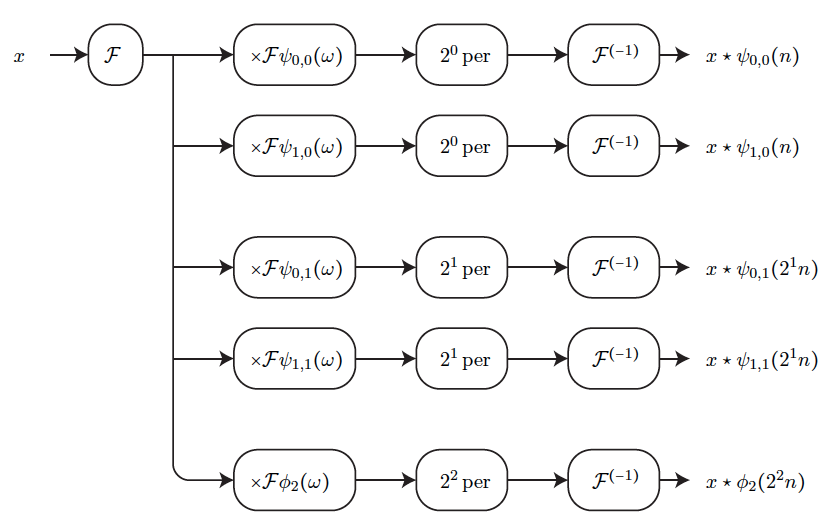
\includegraphics[width=\textwidth]{litreview/images/morlet_fourier_process.png}
      \caption[Fourier Implementation of the Morlet decomposition of an input
              image]
              {Fourier Implementation of the Morlet decomposition of an input
              image, with $J=2$ scales and $L=2$ orientations. The Fourier
              transform of $x$ is calculated and multiplied with the
              (precomputed) Fourier transforms of a bank of Morlet filters. The
              results are periodized according to the target resolution, and
              then the inverse Fourier transform is applied. Image taken from
              \cite{sifre_rigid-motion_2014-1}.}
      \label{fig:ch2:morlet_fourier_process}
  \end{figure}


\subsubsection{Implementation and Efficiency}\label{sec:ch2:dtcwt_efficiency}
  \autoref{fig:ch2:dtcwt_1d_fb} showed the layout for the $\DTCWT$ for 1D signals. We
  saw from \eqref{eq:ch2:dtcwt_2d_product} that the 2D separable product of wavelets
  involved the product of $\psi_g$, $\psi_h$, $\phi_g$, and $\phi_h$ terms, with
  some summing and differencing operations. \autoref{fig:ch2:dtcwt_fb} shows how to
  efficiently implement this with FBs.
  
  \begin{figure}
    \centering
    \makebox[\textwidth][c]{%
      % 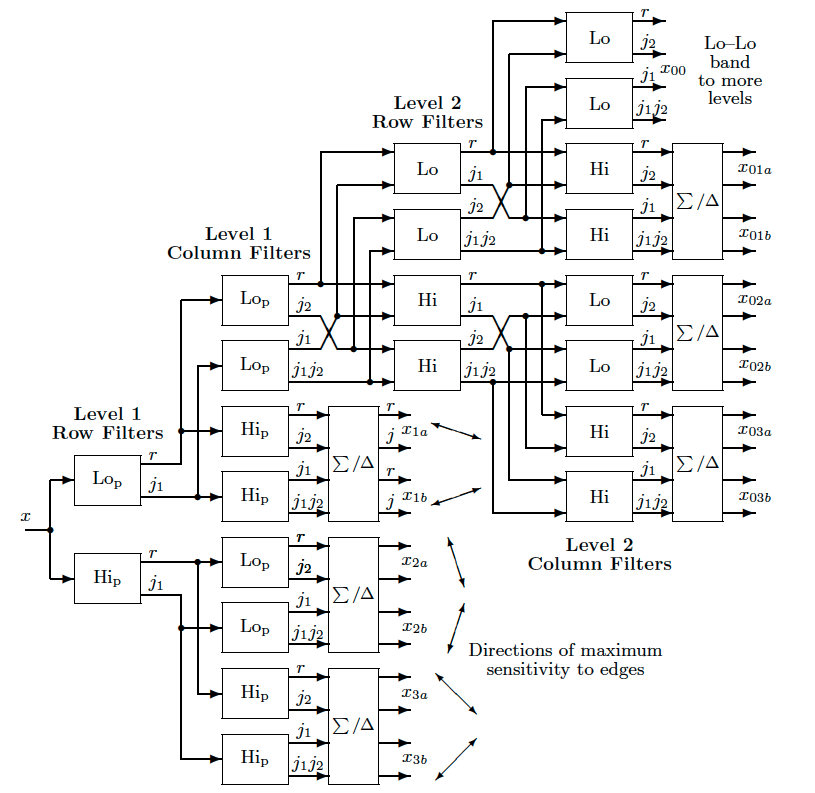
\includegraphics[width=1.1\textwidth]{images/dtcwt_fb.png}
    }
      \caption[The filter bank implementation of the $\DTCWT$]
              {The filter bank implementation of the $\DTCWT$@. Image taken from 
              \cite{kingsbury_image_1999}}
      \label{fig:ch2:dtcwt_fb}
  \end{figure}

  As we did for \autoref{sec:ch2:morlet_implementation}, we calculate and compare
  the complexity of the $\DTCWT$@. To do this, we must know the length of our
  $h$ and $g$ filters. It is also important to know that we must use different
  filters for the first scale to the deeper scales, as this achieves better
  analyticity. A typical configuration will use biorthogonal filters for the
  first scale, then qshift for subsequent scales.
  % The \emph{nearly symmetric type a} biorthogonal filters for the first level, and then the \emph{qshift type b}
  % filters for the deeper levels of the transform. 
  These filters have the following number of taps\footnote{This implementation
  uses the shorter near\_sym\_a biorthogonal filters and qshift\_a filters.
  Smoother wavelets can have slightly more taps}:
  % \begin{table}
    \begin{center}
    \begin{tabular}{ccccc} \hline
                   & $h_0$ & $h_1$ & $g_0$ & $g_1$ \\\hline
      biorthogonal & 5     & 7     & 7     & 5     \\
      qshift       & 10    & 10    & 10    & 10      
    \end{tabular}
    \end{center}
  % \end{table}
  The resulting complexity of the entire forward wavelet transform for an image
  with $N\x N$ pixels is:
  \begin{itemize}
    \item First layer (Image size $=N\x N$):
      \begin{itemize}
        \item Column filtering requires $5N^2+7N^2$ multiply-adds
        \item Row filtering to make the LoLo term requires $5N^2$ more
          multiply-adds
        \item Row filtering to make $15\degs$ and $165\degs$ requires
          $5N^2+4N^2$
          multiply-adds (the 4 here comes from the $\Sigma/\Delta$ function
          block in \autoref{fig:ch2:dtcwt_fb}).
        \item Row filtering to make the $45\degs$ and $135\degs$ requires $7N^2
          +4N^2$ multiply-adds
        \item Row filtering to make the $75\degs and 105\degs$ requires
          $7N^2+4N^2$
          multiply-adds
      \end{itemize}
      The total being 
      $$T(N) = (5+7+5+5+4+7+4+7+4)N^2 = 48N^2$$
    \item Second and deeper layers (Image size $=2^{-j}N\x 2^{-j}N=M\x M$):
      \begin{itemize}
        \item Column filtering requires $10M^2+10M^2$ multiply-adds
        \item Row filtering to make the LoLo term requires $10M^2$ more
          multiply-adds
        \item Row filtering to make $15\degs$ and $165\degs$ requires
          $10M^2+4M^2$
          multiply-adds (the 4 here comes from the $\Sigma/\Delta$ function
          block in \autoref{fig:ch2:dtcwt_fb}).
        \item Row filtering to make the $45\degs$ and $135\degs$ requires
          $10M^2 +4M^2$ multiply-adds
        \item Row filtering to make the $75\degs$ and $105\degs$ requires
          $10M^2+4M^2$
          multiply-adds
      \end{itemize}
      The total being: 
      $$T(M) = (10+10+10+10+4+10+4+10+4)M^2 = 68M = 68\x 2^{-2j}N^2$$
  \end{itemize}
  \begin{equation}
    T(N) = 48N^2 + \sum_{j=1}^{J} 68 \x 2^{-2j}N^2 \approx 100N^2
  \end{equation}
  As the term $\sum_{j=1}^{J} 68 \x 2^{-j}$ is a geometric series that sums to
  $1/3$ as $j \rightarrow \infty$. We have also rounded up the sum to be conservative.

  It is difficult to compare this with the complexity of the Fourier-based
  implementation of the Morlet wavelet transform we have derived in
  \autoref{sec:ch2:morlet_implementation}, as we cannot readily estimate the big-O
  order constants for the 2D FFT method. However, the central term, $JLN^2$,
  would cost $24N^2$ multiplies for four scales and six orientations. These are
  complex multiplies, as they are in the Fourier domain, which requires
  four real multiplies. On top of this, to account for the periodic repetition 
  of the inverse FFT implementation, Mallat et.\ al.\ symmetrically extend the image by
  $N/2$ in each direction. This means that the central term is already on the
  order of $\sim 200N^2$ multiplies, without even considering the more
  expensive forward and inverse FFTs. 

  For a simple comparison experiment, we performed the two transforms on a four
  core Intel i7 processor (a moderately high-end personal computer). The
  $\DTCWT$ transform took roughly 0.15s on a black and
  white $32\x 32$ image, vs. 0.5s for the Fourier-based method. For a larger,
  $512\x 512$ image, the $\DTCWT$ implementation took 0.35s vs. 3.5s
  (times were averaged over several runs).
